\PassOptionsToPackage{hidelinks}{hyperref}
\documentclass[12pt, oneside]{article} 

\usepackage{geometry}
\geometry{tmargin=.75in, bmargin=.75in, lmargin=.75in, rmargin = .75in}  
\usepackage{multicol}
\usepackage{amsmath}
\usepackage{graphicx}
\usepackage{listings}
\usepackage{tikz}
\usepackage{hyperref}
\usepackage{bookmark}
\usepackage{amsfonts}
\usepackage{appendix}


\title{\textbf{Typsetting Academic Manuscripts} \\
~\\
A Practical Introduction to \LaTeX{}}
\author{Derron Borders}
\date{October 25, 2024}

\begin{document}

\maketitle
\newpage
\tableofcontents
\newpage


\section*{Preface}
When I started my master's in linguistics at the University of Utah, I was introduced to \LaTeX{} by a couple of professors. \LaTeX{} is a software system for typesetting documents. \LaTeX{} markup describes the content and layout of the document, as opposed to the formatted text found in What-you-see-is-what-you-get (WYSIWYG) word processors like Google Docs, LibreOffice Writer, and Microsoft Word. 

It was very useful, especially since linguistics uses a lot of special formatting in subfields like syntax and semantics. I used it to format my master's thesis at the U because there was already a U of Utah thesis class and I only had to worry about the writing instead of the formatting. In fact, I continued to use \LaTeX{} throughout my second master's degree at Bowling Green State University because the documents it makes are just so beautiful, compared to those created by Microsoft Word or Google Docs. There are APA 7th Edition classes (as well as many many others) and utilizing BetterBib with Zotero makes incorporating citations a breeze.

I use Visual Studio Code (VSCode) in conjunction with MacTeX, MiKTeX, \LaTeX{} Workshop, Zotero, and BetterBib to organize and prepare my manuscripts. While it may seem like there is a steep learning curve, it has absolutely changed my life and has made the process of writing so much more fun! I am writing this manual (using \LaTeX{} by the way) as a way to help any academic writers who are looking for a way to focus more on writing than on the formatting of their papers. As someone who lives with ADHD, it can be easy to get distracted when writing and I need organization and a process. \LaTeX{} has allowed me to streamline a process for writing that allows me to produce manuscripts with a variety of style parameters (e.g., APA, Chicago, MLA), without having to constantly relearn and verify if my citations, references, footnotes, and endnotes are formatted correctly, due to the various packages available to \LaTeX{} users. 

As a academic in the field of Adult Learning and Leadership, I've designed this manual to be most accessible to those scholars who are not in fields like STEM, linguistics, and other specialized fields that use complex formulas and graphics in their manuscripts. This manual is a general overview of the process I use to create manuscripts for publishing that might include basic tables and figures. While this isn't geared towards those who are in the STEM field, it should still be an accessible introduction to \LaTeX{}. If you are planning on writing a thesis or dissertation, I highly recommend learning \LaTeX{}. 

I do plan on trying to keep this document updated and hopefully adding a glossary and index section to help with navigation. You can click on the section titles in the table of comments to go directly to that section. All URLs are also clickable.

\newpage
\part{Getting Started with \LaTeX{}}

\section{Introduction to \LaTeX{}}\label{intro}

LaTeX (pronounced \textit{LAY-tek} or \textit{LAH-tek}) is a \textbf{document preparation system} used for typesetting high-quality documents, especially those containing complex mathematical equations, technical content, and academic papers.

At its core, LaTeX is a markup language that defines how your content should be formatted, much like HTML or Markdown. Unlike a word processor, where you adjust formatting visually (e.g., changing fonts or margins directly), LaTeX separates \textbf{content} from \textbf{style}. You write your document in a plain text file using LaTeX commands to describe the structure (e.g., sections, equations, or references), and the system compiles it into a polished PDF output.

It was originally developed by Leslie Lamport in the 1980s as an extension of TeX, a typesetting system created by Donald Knuth. Since then, it has become a standard for academic writing in fields such as mathematics, computer science, engineering, and the natural sciences.

\subsection{Why Use \LaTeX{}?}

\LaTeX{} offers several benefits that make it a preferred tool for academics, researchers, and technical writers:

\begin{enumerate}
    \item \textbf{Professional Typesetting and Layout}
    \begin{itemize}
        \item \LaTeX{} excels at producing beautifully formatted text with minimal effort.
        \item It handles complex structures--like footnotes, references, and equations--elegantly and consistently.
        \item Outputs are publication-ready, making it the go-to tool for academic journals and conference papers.
    \end{itemize}
    
    \item \textbf{Superior Handling of Mathematical Content}
    \begin{itemize}
        \item \LaTeX{} is unmatched when it comes to typesetting mathematical symbols, equations, and formulas.
        \item Whether you need simple equations or complex multi-line mathematical expressions, \LaTeX{} renders them precisely.
        \item This makes it especially valuable in fields such as mathematics, physics, and engineering.
    \end{itemize}
    
    \item \textbf{Automated Document Management}
    \begin{itemize}
        \item \LaTeX{} automatically handles references, citations, cross-referencing, table of contents, lists of figures, and bibliographies with ease.
        \item You can focus on writing content without worrying about keeping track of formatting and page layout.
    \end{itemize}

    \item \textbf{Scalability for Large Projects}
    \begin{itemize}
        \item \LaTeX{} is ideal for long documents like dissertations, theses, and books.
        \item It allows you to manage content across multiple files and compile everything into one seamless output.
        \item Collaboration on complex projects is easier, as \LaTeX{} files are plain text and version control friendly (e.g., with Git).
    \end{itemize}

    \item \textbf{Consistency Across Devices}
    \begin{itemize}
        \item Unlike word processors that can behave differently across operating systems, \LaTeX{} ensures consistent formatting regardless of platform.
        \item A \LaTeX{} document compiled on one computer will look identical when compiled on another.
    \end{itemize}

    \item \textbf{Open-Source and Free}
    \begin{itemize}
        \item \LaTeX{} is free to use and has extensive community support.
        \item There are numerous templates available for research papers, theses, CVs, and presentations.
        \item It is supported by tools like Overleaf, a web-based \LaTeX{} editor that facilitates collaboration and online editing.
    \end{itemize}

    \item \textbf{Separation of Content and Formatting}
    \begin{itemize}
        \item With \LaTeX{}, you focus on content creation the system takes care of the formatting based on pre-defined document classes (like \texttt{article} or \texttt{book}).
        \item This separation allows you to maintain consistent styling throughout the document without repetitive formatting work.
    \end{itemize}
\end{enumerate}

\subsection{When Should You Use \LaTeX?}

\LaTeX{} is particularly useful for:
\begin{itemize}
    \item Writing academic papers, research articles, and theses
    \item Creating technical documents with equations, tables, and figures
    \item Producing CVs or resumes with clean and professional layouts
    \item Formatting scientific presentations using Beamer
    \item Writing books or long-form content with structured chapters
\end{itemize}

\subsection{Challenges of Using \LaTeX{}}

While \LaTeX{} offers many benefits, it also comes with a learning curve:
\begin{itemize}
    \item It can feel intimidating for beginners since it relies on commands and coding rather than WYSIWYG (What You See Is What You Get) editing.
    \item Debugging errors can be frustrating, as small syntax mistakes (e.g., a missing bracket) can prevent the document from compiling.
    \item For quick, simple documents, a word processor like Microsoft Word may be more convenient.
\end{itemize}

Despite its initial complexity, \LaTeX{} becomes an invaluable tool once mastered. It provides precise control over document structure and formatting, making it the best choice for academics, researchers, and technical professionals. The time invested in learning \LaTeX{} pays off in terms of polished documents that are well-suited for publication or presentation.

In summary, if you are working on academic, technical, or mathematical content, \LaTeX{} is worth the effort!
\subsection{Comparison with Word Processors (MS Word vs. \LaTeX{})}

When deciding whether to use \LaTeX{} or a traditional word processor like Microsoft Word, it’s helpful to compare the two based on their strengths and limitations. See the Table \ref{tab:comparison} on the next page.
\newpage
\begin{table}[h!]
\centering
\begin{tabular}{|p{4cm}|p{6cm}|p{6cm}|}
\hline
\textbf{Aspect} & \textbf{Microsoft Word} & \textbf{\LaTeX{}} \\ 
\hline
\textbf{Ease of Use} & 
WYSIWYG interface (What You See Is What You Get). 
Ideal for beginners with little to no learning curve. &
Markup-based language; requires learning \LaTeX{} commands. 
Can be intimidating for beginners but offers more flexibility once mastered. \\ 
\hline
\textbf{Formatting Control} & 
Limited control over advanced layout formatting; changes are made manually. &
Precise and automated formatting. Handles complex layouts like equations, tables, and references consistently. \\ 
\hline
\textbf{Mathematical Equations} & 
Basic support for simple equations via built-in equation editor. 
Not ideal for complex mathematical typesetting. &
Designed for professional-quality mathematical typesetting, including multi-line equations and matrices. \\ 
\hline
\textbf{Document Length} & 
Struggles with large documents (theses, books); prone to lag or crashes with many references and figures. & 
Handles long documents efficiently; ideal for theses, books, and multi-file projects with cross-references. \\ 
\hline
\textbf{Collaboration} & 
Good for real-time collaboration through cloud services like OneDrive. 
Issues with version control and merging changes. & 
Supports collaboration through Overleaf or Git-based version control. Text-based files make it easy to track changes. \\ 
\hline
\textbf{References and Bibliography} & 
Manual citation management or use of third-party tools (e.g., EndNote). 
Can be tedious to manage references. & 
Uses BibTeX or BibLaTeX to automate citations and bibliography management. Cross-referencing is seamless. \\ 
\hline
\textbf{Consistency Across Devices} & 
Formatting may vary depending on device, operating system, or Word version. &
Ensures identical output regardless of device or platform. Compiled PDF will look the same everywhere. \\ 
\hline
\textbf{Cost} & 
Requires a paid Microsoft Office license. &
Free and open-source. \\ 
\hline
\end{tabular}
\caption{Comparison of Microsoft Word and \LaTeX{}}
\label{tab:comparison}
\end{table}
\newpage

\section{Setting Up Your \LaTeX{} Environment}

Before you can begin using \LaTeX{}, you need to install a \textbf{LaTeX distribution} and choose a suitable \textbf{LaTeX editor}. This section gives an overview of distributions and editors. Utilize the directions for each program in order to install it on your computer.

\subsection{Installing \LaTeX{} Distributions}

A \LaTeX{} distribution provides all the tools necessary to compile \LaTeX{} code into a PDF. Below are some of the most popular distributions:

\begin{itemize}
    \item \textbf{TeX Live} (Windows, macOS, Linux)  
    The most widely-used distribution, especially on Linux systems.  
    \url{https://www.tug.org/texlive/}
    
    \item \textbf{MiKTeX} (Windows)  
    A lightweight distribution preferred on Windows platforms. It downloads required packages on the fly.  
    \url{https://miktex.org/}
    
    \item \textbf{MacTeX} (macOS)  
    A complete distribution for macOS, including TeX Live and additional tools like TeXShop.  
    \url{https://tug.org/mactex/}
\end{itemize}

After installation, you may need to update the distribution to ensure you have the latest packages and tools.

\subsection{Choosing a \LaTeX{} Editor}

Once your \LaTeX{} distribution is installed, you need an editor to write your \LaTeX{} code. Here are some popular options:

\begin{itemize}
    \item \textbf{Overleaf} (Web-based)  
    A cloud-based platform that allows you to write and compile \LaTeX{} documents online. Great for collaboration and doesn’t require local installation.  
    \url{https://www.overleaf.com/}

    \item \textbf{TeXShop} (macOS)  
    A simple and easy-to-use editor bundled with MacTeX. It offers a straightforward environment for writing and compiling \LaTeX{} documents.

    \item \textbf{TeXstudio} (Windows, macOS, Linux)  
    A cross-platform editor with a lot of built-in features, such as syntax highlighting and auto-completion. Ideal for intermediate users.  
    \url{https://www.texstudio.org/}

    \item \textbf{VSCode with LaTeX Workshop Extension} (Windows, macOS, Linux)  
    A powerful code editor that can be extended with the \LaTeX{} Workshop extension, providing an integrated writing and compiling experience.  
    \url{https://code.visualstudio.com/}
\end{itemize}

\section{Your First LaTeX Document: Hello World}

\subsection{Overview}
Creating your first \LaTeX{} document is a great way to get familiar with the basics. In this section, I’ll walk through the steps required to write and compile a basic \LaTeX{} document that displays the message: \textbf{Hello, world!}

\subsection{Step 1: Create a New \LaTeX{} File}
Follow these steps to create your first \LaTeX{} document:

\begin{enumerate}
    \item Open your \LaTeX{} editor (Overleaf, TeXstudio, TeXShop, or VSCode).
    \item Create a new file and name it \texttt{hello\_world.tex}.
    \item Type the following code into the new file:
\end{enumerate}

\begin{verbatim}
\documentclass{article}
\begin{document}
Hello, world!
\end{document}
\end{verbatim}

\subsection{Explanation of the Code}
Here’s a breakdown of the components used in this simple \LaTeX{} document:

\begin{itemize}
    \item \texttt{\textbackslash documentclass\{article\}}: This command specifies the type of document. Here, we use the \texttt{article} class, which is ideal for shorter documents such as papers, assignments, or reports.
    \item \texttt{\textbackslash begin\{document\} ... \textbackslash end\{document\}}: The content of your document goes between these two commands.
    \item \texttt{Hello, world!}: This is the content that will appear in the PDF output.
\end{itemize}

\subsection{Step 2: Compile the Document}
After typing the code, save the file and compile it to generate a PDF. The steps to compile will vary depending on the editor you are using:

\begin{enumerate}
    \item In \textbf{Overleaf}: Click the \textbf{Recompile} button.
    \item In \textbf{TeXstudio}, \textbf{TexShop}, and \textbf{VSCode}: Click the \textbf{Compile} or \textbf{Build} button.  
    \item Alternatively, you can compile from the command line by opening a terminal and typing:
\end{enumerate}

\begin{verbatim}
pdflatex hello_world.tex
\end{verbatim}

\subsection{Step 3: View the Output}
After successful compilation, you should see a PDF with the following text:

\begin{center}
\textbf{Hello, world!}
\end{center}

\subsection{Troubleshooting}
If your document doesn’t compile successfully, try the following troubleshooting tips:

\begin{itemize}
    \item Make sure all braces \{\} and parentheses are properly closed.
    \item Ensure the file is saved with the \texttt{.tex} extension.
    \item Verify that your \LaTeX{} distribution (such as TeX Live, MiKTeX, or MacTeX) is correctly installed.
\end{itemize}

Congratulations! You’ve successfully created and compiled your first \LaTeX{} document. This simple example demonstrates the core structure of a \LaTeX{} file. In the upcoming sections, we will explore more advanced features and formatting options to help you create professional academic documents.

\section{Anatomy of a \LaTeX{} Document}

Every \LaTeX{} document follows a well-defined structure. Understanding the anatomy of a \LaTeX{} document helps you organize your writing efficiently and make use of \LaTeX’s powerful typesetting features. In this section, we will explore the essential components of a \LaTeX{} document, including document classes, the preamble, and the document structure.

\subsection{Document Classes (article, report, book, etc.)}

The \texttt{documentclass} command defines the type of document you are creating. It influences the overall layout, margins, section formatting, and font sizes. Commonly used document classes include:

\begin{itemize}
    \item \textbf{article}: Used for shorter documents such as research papers, essays, and assignments.
    \item \textbf{report}: Suitable for longer documents like technical reports, theses, or project documentation.
    \item \textbf{book}: Ideal for books or very long documents with chapters and sections.
    \item \textbf{letter}: Used for typesetting formal letters.
    \item \textbf{beamer}: Used for presentations.
\end{itemize}

Example of using the \texttt{article} class:
\begin{verbatim}
\documentclass{article}
\end{verbatim}

You can also customize the document class by adding options in square brackets. For example:
\begin{verbatim}
\documentclass[12pt, a4paper]{report}
\end{verbatim}
This example sets the font size to 12 points and the paper size to A4.

\subsection{Preamble: Packages and Document Settings}

The preamble is the section of the \LaTeX{} document that appears before the \texttt{\textbackslash begin\{document\}} command. In this part, you can load additional packages, set document options, and define custom commands. Below are some common elements of the preamble.

\subsubsection{Loading Packages}

Packages extend \LaTeX’s functionality. Some commonly used packages include:

\begin{itemize}
    \item \texttt{amsmath}: Provides advanced mathematical features.
    \item \texttt{graphicx}: Allows you to include images.
    \item \texttt{hyperref}: Makes URLs and references clickable.
\end{itemize}

Example of loading packages:
\begin{verbatim}
\usepackage{amsmath}
\usepackage{graphicx}
\usepackage{hyperref}
\end{verbatim}

\subsubsection{Customizing Document Settings}

You can adjust layout settings in the preamble. For example, the \texttt{geometry} package allows you to modify margins:
\begin{verbatim}
\usepackage[margin=1in]{geometry}
\end{verbatim}

You can also define your own commands and environments:
\begin{verbatim}
\newcommand{\boldit}[1]{\textbf{\textit{#1}}}
\end{verbatim}
This command creates a shortcut to make text both bold and italic.

\subsection{Structure: Title, Abstract, Sections, and Paragraphs}

The content of your document is enclosed between the \texttt{\textbackslash begin\{document\}} and \texttt{\textbackslash end\{document\}} commands. Inside this environment, you organize your content using sections, paragraphs, and additional formatting elements.

\subsubsection{Title and Author Information}

You can add a title, author name, and date using the following commands:
\begin{verbatim}
\title{My First \LaTeX{} Document}
\author{John Doe}
\date{\today}
\end{verbatim}

Use the \texttt{\textbackslash maketitle} command to generate the title block in the document:
\begin{verbatim}
\begin{document}
\maketitle
\end{document}
\end{verbatim}

\subsubsection{Abstract}

The abstract provides a brief summary of the document. It is placed inside the \texttt{abstract} environment:
\begin{verbatim}
\begin{abstract}
This is a brief summary of the document.
\end{abstract}
\end{verbatim}

\subsubsection{Sections and Subsections}

Use sections and subsections to organize your document. \LaTeX{} automatically numbers the sections and generates a table of contents if required.

\begin{verbatim}
\section{Introduction}
This is the introduction.

\subsection{Background}
This is the background section.

\subsubsection{Details}
This section contains more detailed information.
\end{verbatim}

\subsubsection{Paragraphs and Line Breaks}

Separate paragraphs with a blank line. If you need a line break without starting a new paragraph, use \texttt{\textbackslash\textbackslash}:
\begin{verbatim}
This is the first line.\\
This is the second line after a line break.
\end{verbatim}

\subsection{Complete Example: Basic \LaTeX{} Document}

Here is a complete example of a simple \LaTeX{} document:

\begin{verbatim}
\documentclass{article}
\usepackage{amsmath}
\usepackage{graphicx}
\usepackage{hyperref}

\title{Anatomy of a \LaTeX{} Document}
\author{Jane Smith}
\date{\today}

\begin{document}

\maketitle

\begin{abstract}
This document provides an overview of the structure of a basic \LaTeX{} document.
\end{abstract}

\section{Introduction}
\LaTeX{} is a powerful tool for typesetting documents.

\subsection{Background}
This section provides background information.

\subsubsection{Details}
Detailed information goes here.

\section{Conclusion}
This is the conclusion of the document.

\end{document}
\end{verbatim}

\subsection*{Conclusion}

The anatomy of a \LaTeX{} document consists of three main parts: the document class, the preamble, and the main content. Understanding how these components work will help you structure and organize your documents efficiently. In the next sections, we will explore more advanced formatting options and \LaTeX{} features.

\section{Typesetting a Manuscript Using the apa7 Class}

The \texttt{apa7} document class is designed to follow the formatting guidelines of the American Psychological Association (APA) 7th Edition. It provides an easy way to create APA-compliant papers, including proper margins, font sizes, headings, and reference management. This section explains how to use the \texttt{apa7} class to typeset a manuscript.

\subsection{Installing the apa7 Class}

Most \LaTeX{} distributions (such as TeX Live, MiKTeX, and MacTeX) come with the \texttt{apa7} class pre-installed. If you encounter errors related to the class not being found, try updating your \LaTeX{} distribution or manually installing the class by running:
\begin{verbatim}
tlmgr install apa7  % For TeX Live
\end{verbatim}

\subsection{Using the apa7 Document Class}

To use the \texttt{apa7} class, declare it at the beginning of your document with:
\begin{verbatim}
\documentclass[man]{apa7}
\end{verbatim}
The \texttt{man} option specifies that the document is a manuscript. Other options include:
\begin{itemize}
    \item \texttt{jou}: For journal submissions.
    \item \texttt{doc}: For documents (e.g., term papers).
    \item \texttt{12pt}: For font size (default is 12pt).
\end{itemize}

\subsection{Preamble: Essential Packages for APA Formatting}

In addition to the \texttt{apa7} class, you may need to load some useful packages:
\begin{verbatim}
\usepackage{csquotes}    % For proper quotation formatting
\usepackage[backend=biber,style=apa]{biblatex} % APA-style bibliography
\addbibresource{references.bib} % Bibliography file
\end{verbatim}
The \texttt{csquotes} package ensures proper quotation marks, and \texttt{biblatex} allows APA-style citation management.

\subsection{Title Page, Abstract, and Main Body}

Below is an example structure of an APA-compliant manuscript using the \texttt{apa7} class.

\begin{verbatim}
\documentclass[man]{apa7}
\usepackage{csquotes}
\usepackage[backend=biber,style=apa]{biblatex}
\addbibresource{references.bib}

\title{An Example APA Manuscript}
\shorttitle{APA Manuscript}
\author{John Doe}
\affiliation{University of Example}
\authornote{This research was supported by...}

\abstract{
This is a sample abstract. It provides a brief overview of the research
topic, methods, and findings. Abstracts should be concise and informative.
}

\begin{document}

\maketitle

\section{Introduction}
The introduction explains the background of the study and its objectives.
In-text citations should follow the APA format,for example: 
\textcite{doe2020} argues that...

\section{Method}
The method section describes the research design, participants, procedures,
and measures used in the study.

\section{Results}
The results section presents the findings of the study. Statistical results 
should follow APA guidelines.

\section{Discussion}
The discussion interprets the results, relates them to previous research,
and suggests future directions.

\printbibliography

\end{document}
\end{verbatim}

\subsection{Explanation of Key Components}

\begin{itemize}
    \item \texttt{\textbackslash title}: Specifies the title of the manuscript.
    \item \texttt{\textbackslash shorttitle}: Provides a shortened version of the title for running heads.
    \item \texttt{\textbackslash author} and \texttt{\textbackslash affiliation}: Lists the author’s name and institutional affiliation.
    \item \texttt{\textbackslash authornote}: Adds a note about funding, acknowledgments, or conflicts of interest.
    \item \texttt{\textbackslash abstract}: Defines the abstract.
    \item \texttt{\textbackslash maketitle}: Generates the title page.
    \item \texttt{\textbackslash printbibliography}: Outputs the bibliography based on the BibTeX file.
\end{itemize}

\subsection{Citations and References}

The \texttt{biblatex} package allows you to manage APA-style references easily. Add your references in a \texttt{references.bib} file:
\begin{verbatim}
@article{doe2020,
  author = {Doe, John},
  title = {A Study on Sample Manuscripts},
  journal = {Journal of Example Research},
  year = {2020},
  volume = {15},
  number = {3},
  pages = {23-45},
  doi = {10.xxxx/journal.2020}
}
\end{verbatim}

You can cite this reference in the document using:
\begin{verbatim}
\textcite{doe2020}
\end{verbatim}

\subsection{Formatting and Submissions}

The \texttt{apa7} class ensures proper APA formatting for margins, font size, line spacing, and section headings. For journal or class submissions, make sure to follow any additional guidelines provided by the institution or publisher.

\subsection*{Conclusion}

Using the \texttt{apa7} class simplifies the process of creating APA-compliant manuscripts. With features such as automatic formatting, sectioning, and bibliography management, \LaTeX{} offers a powerful tool for students, researchers, and authors following APA guidelines.

\part{Essential \\LaTeX{} Features}

\section{Working with Text and Fonts}

\LaTeX{} provides extensive options for formatting text and customizing fonts. This section will guide you through the basics of text formatting, working with lists, and customizing fonts and layouts to meet your document’s needs.

\subsection{Basic Text Formatting: Italics, Bold, and Underlines}

Here are the most common ways to format text in \LaTeX{}:

\begin{itemize}
    \item \textbf{Italics:} Use the \texttt{\textbackslash textit\{...\}} command to italicize text.
    \item \textbf{Bold:} Use the \texttt{\textbackslash textbf\{...\}} command for bold text.
    \item \textbf{Underline:} Use the \texttt{\textbackslash underline\{...\}} command to underline text.
\end{itemize}

Example:
\begin{verbatim}
This is \textit{italicized} text. 
This is \textbf{bold} text. 
This is \underline{underlined} text.
\end{verbatim}

The output will appear as:

This is \textit{italicized} text.  
This is \textbf{bold} text.  
This is \underline{underlined} text.

\subsubsection{Combining Multiple Styles}
You can combine different styles by nesting commands:
\begin{verbatim}
This is \textbf{\textit{bold and italicized}} text.
\end{verbatim}

The output will be:

This is \textbf{\textit{bold and italicized}} text.

\subsection{Lists (Itemized, Enumerated, and Descriptions)}

\LaTeX{} provides several list environments to organize content.

\subsubsection{Itemized Lists}
Use the \texttt{itemize} environment to create bulleted lists:
\begin{verbatim}
\begin{itemize}
    \item First item
    \item Second item
\end{itemize}
\end{verbatim}

Output:

\begin{itemize}
    \item First item
    \item Second item
\end{itemize}

\subsubsection{Enumerated Lists}
Use the \texttt{enumerate} environment to create numbered lists:
\begin{verbatim}
\begin{enumerate}
    \item First item
    \item Second item
\end{enumerate}
\end{verbatim}

Output:

\begin{enumerate}
    \item First item
    \item Second item
\end{enumerate}

\subsubsection{Description Lists}
The \texttt{description} environment allows for labeled lists:
\begin{verbatim}
\begin{description}
    \item[First] Description of the first item.
    \item[Second] Description of the second item.
\end{description}
\end{verbatim}

Output:

\begin{description}
    \item[First] Description of the first item.
    \item[Second] Description of the second item.
\end{description}

\subsection{Customizing Fonts and Layout Styles}

\LaTeX{} allows you to change fonts and layouts to customize your document.

\subsubsection{Changing the Font Family}
You can switch between different font families using the following commands:
\begin{verbatim}
\textrm{Roman family}   % Default serif font
\textsf{Sans-serif}     % Sans-serif font
\texttt{Monospace}      % Monospace font
\end{verbatim}

Output:

\textrm{Roman family}  
\textsf{Sans-serif}  
\texttt{Monospace}

\subsubsection{Changing Font Size}
Font size can be set globally or locally.

\textbf{Global Font Size:} Set in the document class:
\begin{verbatim}
\documentclass[12pt]{article}
\end{verbatim}

\textbf{Local Font Size:} Use the following commands:
\begin{verbatim}
{\tiny Tiny text}
{\small Small text}
{\normalsize Normal text}
{\large Large text}
{\Huge Huge text}
\end{verbatim}

Output:

{\tiny Tiny text}  
{\small Small text}  
{\normalsize Normal text}  
{\large Large text}  
{\Huge Huge text}

\subsubsection{Customizing Fonts with Packages}
You can change the fonts in your document by loading packages in the preamble:

\begin{verbatim}
\usepackage{times}     % Use Times New Roman
\usepackage{helvet}    % Use Helvetica
\usepackage{courier}   % Use Courier
\end{verbatim}

If you need more font options, consider using the \texttt{fontspec} package (for XeLaTeX or LuaLaTeX):
\begin{verbatim}
\usepackage{fontspec}
\setmainfont{Georgia}  % Use Georgia font
\end{verbatim}

\subsubsection{Line Spacing and Paragraph Layout}
Use the \texttt{setspace} package to adjust line spacing:
\begin{verbatim}
\usepackage{setspace}
\onehalfspacing  % 1.5 line spacing
\end{verbatim}

Control paragraph indentation and spacing with these commands:
\begin{verbatim}
\setlength{\parindent}{0pt}   % No indentation
\setlength{\parskip}{10pt}    % 10pt space between paragraphs
\end{verbatim}

\subsubsection{Customizing Headers and Footers}
The \texttt{fancyhdr} package allows you to customize headers and footers:
\begin{verbatim}
\usepackage{fancyhdr}
\pagestyle{fancy}
\fancyhead[L]{Left Header}  % Left-aligned header
\fancyhead[C]{Center Header}  % Centered header
\fancyhead[R]{Right Header}  % Right-aligned header
\fancyfoot[C]{\thepage}  % Centered page number in footer
\end{verbatim}

\subsection*{Conclusion}

\LaTeX{} offers powerful tools for text formatting and layout customization. With the ability to manage lists, change fonts, and adjust layouts, you can produce professional-looking documents tailored to your needs. In the next sections, we will explore advanced features, including tables, figures, and mathematical content.

\section{Including Tables and Figures}

Tables and figures are essential components of many documents, especially academic papers. \LaTeX{} provides flexible environments for creating, positioning, and referencing tables and figures. This section will guide you through using the \texttt{tabular} environment for tables, adding captions to figures, and properly referencing them within your document.

\subsection{Creating Tables with \texttt{tabular}}

The \texttt{tabular} environment is used to create simple tables. You can specify the alignment of columns and use vertical and horizontal lines to structure the table.

\subsubsection{Basic Table Example}

Here is a simple 2x2 table with left-aligned columns and horizontal borders:
\begin{verbatim}
\begin{tabular}{|l|l|}
\hline
Item & Description \\ \hline
Apples & Red or green fruit \\ \hline
Bananas & Yellow fruit \\ \hline
\end{tabular}
\end{verbatim}

Output:

\begin{tabular}{|l|l|}
\hline
Item & Description \\ \hline
Apples & Red or green fruit \\ \hline
Bananas & Yellow fruit \\ \hline
\end{tabular}

\subsubsection{Column Alignment}

You can align columns to the left (\texttt{l}), center (\texttt{c}), or right (\texttt{r}). Use \texttt{|} to add vertical borders between columns.

Example:
\begin{verbatim}
\begin{tabular}{|c|r|l|}
\hline
Center & Right & Left \\ \hline
1 & 2 & 3 \\ \hline
\end{tabular}
\end{verbatim}

\begin{tabular}{|c|r|l|}
\hline
Center & Right & Left \\ \hline
1 & 2 & 3 \\ \hline
\end{tabular}

\subsubsection{Adding Captions and Labels to Tables}

Use the \texttt{table} environment to add captions and labels for referencing:
\begin{verbatim}
\begin{table}[h]
\centering
\begin{tabular}{|l|l|}
\hline
Item & Description \\ \hline
Apples & Red or green fruit \\ \hline
Bananas & Yellow fruit \\ \hline
\end{tabular}
\caption{A sample fruit table}
\label{tab:fruit}
\end{table}
\end{verbatim}

\begin{table}[h]
\centering
\begin{tabular}{|l|l|}
\hline
Item & Description \\ \hline
Apples & Red or green fruit \\ \hline
Bananas & Yellow fruit \\ \hline
\end{tabular}
\caption{A sample fruit table}
\label{tab:fruit}
\end{table}

\subsection{Positioning and Captioning Figures}

Figures can be included using the \texttt{figure} environment with the \texttt{graphicx} package. This allows you to position, caption, and reference figures effectively.

\subsubsection{Including an Image}

Use the \texttt{\textbackslash includegraphics} command to include an image:
\begin{verbatim}
\usepackage{graphicx}

\begin{figure}[h]
\centering
\includegraphics[width=0.5\textwidth]{example-image.png}
\caption{Sample figure with caption}
\label{fig:sample}
\end{figure}
\end{verbatim}

This code adds a figure centered on the page, scales it to half the text width, and includes a caption and label.

\subsubsection{Positioning Figures}

You can control the placement of figures using placement specifiers:
\begin{itemize}
    \item \texttt{h}: Place the figure \textbf{here}, at the current location.
    \item \texttt{t}: Place the figure at the \textbf{top} of the page.
    \item \texttt{b}: Place the figure at the \textbf{bottom} of the page.
    \item \texttt{p}: Place the figure on a \textbf{separate} page for floats (figures or tables).
\end{itemize}

Example:
\begin{verbatim}
\begin{figure}[t]
\centering
\includegraphics[width=\textwidth]{example-image.png}
\caption{A figure at the top of the page}
\label{fig:topfigure}
\end{figure}
\end{verbatim}

\subsection{Referencing Figures and Tables in Text}

\LaTeX{} makes it easy to reference tables and figures. Use the \texttt{\textbackslash label} command inside the \texttt{table} or \texttt{figure} environment and the \texttt{\textbackslash ref} or \texttt{\textbackslash autoref} command to refer to them in your text.

Example:
\begin{verbatim}
As shown in Table \ref{tab:fruit}, apples are a common fruit.
\end{verbatim}

Output:  
As shown in Table \ref{tab:fruit}, apples are a common fruit.

Similarly, you can reference figures:
\begin{verbatim}
Figure \ref{fig:sample} illustrates the sample image used.
\end{verbatim}

Output:  
Figure 1 illustrates the sample image used.

\subsubsection{Using \texttt{\textbackslash autoref} for Automatic Labels}

The \texttt{hyperref} package allows you to use \texttt{\textbackslash autoref}, which automatically inserts the appropriate label (e.g., ``Figure", ``Table"):
\begin{verbatim}
\usepackage{hyperref}

As shown in \autoref{tab:fruit}, apples are a common fruit.
\end{verbatim}

Output:  
As shown in \autoref{tab:fruit}, apples are a common fruit.

\subsection*{Conclusion}

Tables and figures are crucial elements in many documents. \LaTeX{} provides powerful tools to structure, position, and reference them accurately. The \texttt{tabular} and \texttt{figure} environments allow you to create professional-looking tables and figures with captions and labels. In the next section, we will explore how to manage citations and bibliographies effectively.

\section{Citations and Bibliography Management}

\LaTeX{} provides powerful tools to manage citations and bibliographies, making it easy to reference academic works and produce properly formatted bibliographies. This section will cover the use of `\textbackslash cite' and `\textbackslash bibitem' for simple references, as well as managing references using the more advanced `biblatex' package with the `biber' backend. We will also explore formatting options for popular citation styles like APA, IEEE, and Chicago.

\subsection{Using \texttt{\textbackslash cite} and \texttt{\textbackslash bibitem} for References}

The simplest way to add citations in \LaTeX{} is by using the `thebibliography' environment with `\textbackslash cite' and `\textbackslash bibitem' entry corresponds to a reference, which can be cited in the text using the `\textbackslash cite' command.

\subsubsection{Example of thebibliography Environment}

Here is an example of how to use `\textbackslash thebibliography' and `\textbackslash bibitem':
\begin{verbatim}
\begin{thebibliography}{99}

\bibitem{lamport1994}
  Lamport, L. (1994). 
  \textit{\LaTeX{}: A Document Preparation System}. 
  Addison-Wesley.

\bibitem{knuth1986}
  Knuth, D. E. (1986). 
  \textit{The TeXbook}. 
  Addison-Wesley.

\end{thebibliography}
\end{verbatim}

To cite one of the references in the text, use the `\cite' command:
\begin{verbatim}
Lamport developed \LaTeX{} \cite{lamport1994}.
\end{verbatim}

Output:  
Lamport developed \LaTeX{} \cite{lamport1994}.

While this method is simple, it becomes difficult to manage when working with many references. For larger projects, it is recommended to use BibTeX or `biblatex'.

\subsection{Managing References with BibTeX and BibLaTeX}

BibTeX and `biblatex' offer more powerful ways to manage bibliographies. BibTeX uses `.bib' files to store references, while `biblatex' (with `biber' as its backend) provides more flexibility and customization.

\subsubsection{Creating a .bib File}

A `.bib' file contains bibliographic information for all references in your document. Here is an example of a `.bib' file named `references.bib':

\begin{verbatim}
@book{lamport1994,
  author    = {Leslie Lamport},
  title     = {LaTeX: A Document Preparation System},
  year      = {1994},
  publisher = {Addison-Wesley}
}

@book{knuth1986,
  author    = {Donald E. Knuth},
  title     = {The TeXbook},
  year      = {1986},
  publisher = {Addison-Wesley}
}
\end{verbatim}

\subsubsection{Using BibTeX with \LaTeX{}}

To use BibTeX, follow these steps:

\begin{enumerate}



\item Include the following commands in your LaTeX document:\\
   \begin{verbatim}
   \bibliographystyle{plain}
   \bibliography{references}
   \end{verbatim}
\item Compile the document using:
\begin{enumerate}
   \item `pdflatex'
   \item `bibtex'
   \item `pdflatex' (twice)
\end{enumerate}
\end{enumerate}

The `plain' style produces a numeric bibliography, but you can change the style to `ieeetr', `apalike', or other formats.

\subsection{Using biblatex with Biber}

The `biblatex' package offers greater control over citations and bibliography formatting. It works with `biber' as its backend for better compatibility with modern citation styles.

\subsubsection{Setting Up BibLaTeX and Biber}


\begin{enumerate}


\item Include the `biblatex' package in the preamble:\\
   \begin{verbatim}
   \usepackage[backend=biber,style=apa]{biblatex}
   \addbibresource{references.bib}
   \end{verbatim}

\item Compile the document using:
 \begin{enumerate}


   \item `pdflatex'
   \item `biber'
   \item `pdflatex' (twice)
\end{enumerate}
\end{enumerate}

The `backend=biber' option ensures that the bibliography is processed using `biber', and the `style=apa' option applies the APA citation style. Other styles include `ieee' and `chicago'.

\subsubsection{Citing References with biblatex}

Biblatex has different citation commands to cite references. For example, you can use the `\textbackslash cite' and `\textbackslash textcite' commands to cite references in different ways:

\begin{verbatim}
According to \textcite{lamport1994}, LaTeX is a powerful tool.
It is also discussed in other texts \cite{knuth1986}.
\end{verbatim}

Output:  
According to Lamport (1994), LaTeX is a powerful tool.  
It is also discussed in other texts (Knuth, 1986).\\

You can find a cheatsheet for biblatex in the following document: \url{https://tug.ctan.org/info/biblatex-cheatsheet/biblatex-cheatsheet.pdf}

\subsubsection{Printing the Bibliography}

Use the `\textbackslash printbibliography' command to print the bibliography:
\begin{verbatim}
\printbibliography
\end{verbatim}

\subsection{Formatting the Bibliography (APA, IEEE, Chicago, etc.)}

The `biblatex' package supports various citation styles. Here are some examples:

\begin{itemize}
    \item \textbf{APA Style:}
    \begin{verbatim}
    \usepackage[backend=biber,style=apa]{biblatex}
    \end{verbatim}
    This style is used for social sciences and follows APA 7th edition guidelines.

    \item \textbf{IEEE Style:}
    \begin{verbatim}
    \usepackage[backend=biber,style=ieee]{biblatex}
    \end{verbatim}
    IEEE style is commonly used in technical and engineering fields.

    \item \textbf{Chicago Style:}
    \begin{verbatim}
    \usepackage[backend=biber,style=chicago-authordate]{biblatex}
    \end{verbatim}
    Chicago style is popular in humanities and follows the author-date format.
\end{itemize}

\subsection{Troubleshooting Tips}

If your bibliography is not displaying correctly, try the following:

\begin{itemize}
    \item Ensure the `.bib' file is in the same directory as your \LaTeX{} document.
    \item Run `biber' instead of `bibtex' if you are using `biblatex'.
    \item Compile the document multiple times to update cross-references.
    \item Check the log file for errors related to bibliography compilation.
\end{itemize}

\subsection*{Conclusion}

Managing citations and bibliographies in \LaTeX{} can be done using `thebibliography' for simple projects or BibTeX and `biblatex' for more complex documents. Using `biblatex' with `biber' provides greater control and supports a wide range of citation styles such as APA, IEEE, and Chicago. With the proper setup, \LaTeX{} can handle all your citation and referencing needs efficiently.


\part{Formatting Academic Manuscripts}

\section{Structuring a Large Document}

When working on large documents like theses, reports, or books, \LaTeX{} offers powerful tools to organize the structure. This section covers how to use chapter and sectioning commands, generate a table of contents, lists of figures and tables, and create appendices.

\subsection{Chapter and Sectioning Commands}

\LaTeX{} provides hierarchical commands to divide your document into sections. The most common ones are:

\begin{itemize}
    \item \texttt{\textbackslash part}: Divides the document into major parts (used in books).
    \item \texttt{\textbackslash chapter}: Used for chapters (only in the \texttt{report} or \texttt{book} class).
    \item \texttt{\textbackslash section}: Creates a new section.
    \item \texttt{\textbackslash subsection}: Creates a subsection under a section.
    \item \texttt{\textbackslash subsubsection}: Creates a smaller subsection.
    \item \texttt{\textbackslash paragraph} and \texttt{\textbackslash subparagraph}: For even finer divisions.
\end{itemize}

Example:
\begin{verbatim}
\chapter{Introduction}
This is the first chapter.

\section{Background}
This section provides background information.

\subsection{Previous Research}
This subsection covers related work.

\subsubsection{Key Findings}
Detailed information goes here.
\end{verbatim}

Each section will be numbered automatically, and \LaTeX{} will manage the hierarchy of the headings for you.

\subsection{Table of Contents, List of Figures, and List of Tables}

In longer documents, it is essential to provide a table of contents (ToC) and lists for figures and tables. \LaTeX{} makes it easy to generate these automatically.

\subsubsection{Table of Contents}
Include the following command where you want the table of contents to appear:
\begin{verbatim}
\tableofcontents
\end{verbatim}

The table of contents will include all chapters, sections, and subsections by default. It is typically placed after the title page.

\subsubsection{List of Figures and List of Tables}
To generate lists of figures and tables, use the following commands:
\begin{verbatim}
\listoffigures
\listoftables
\end{verbatim}

These lists will include all figures and tables in the document along with their captions and page numbers.

\subsubsection{Updating the Table of Contents, Figures, and Tables}
If you make changes to the document structure, recompile the document twice to ensure that the ToC, list of figures, and list of tables are updated correctly.

\subsection{Creating Appendices}

Appendices are used to include supplementary information at the end of the document. In \LaTeX{}, you can create appendices using the \texttt{appendix} environment or the \texttt{\textbackslash appendix} command.

\subsubsection{Using the \texttt{appendix} Command}
The simplest way to create appendices is by using the \texttt{\textbackslash appendix} command, which changes the sectioning to start with ``Appendix" instead of a chapter or section number.

Example:
\begin{verbatim}
\appendix

\chapter{Additional Data}
This appendix contains extra data.

\section{Details of the Experiment}
Here are further details about the experiment.
\end{verbatim}

\subsubsection{Using the \texttt{appendices} Environment}
The \texttt{appendices} package provides additional formatting options for appendices. Load it in the preamble:
\begin{verbatim}
\usepackage{appendix}
\end{verbatim}

Then use the \texttt{appendices} environment:
\begin{verbatim}
\begin{appendices}
    \section{First Appendix}
    This is the first appendix.

    \section{Second Appendix}
    This is the second appendix.
\end{appendices}
\end{verbatim}

\subsection{Cross-Referencing Chapters, Sections, and Appendices}

\LaTeX{} makes it easy to reference different parts of your document. Use the \texttt{\textbackslash label} command to label sections, figures, or tables, and the \texttt{\textbackslash ref} command to refer to them.

Example:
\begin{verbatim}
\chapter{Introduction}
\label{ch:intro}

As discussed in Chapter \ref{ch:intro}, this is the introduction.
\end{verbatim}

Output:  
As discussed in Section \ref{intro}, this is the introduction.

\subsection{Putting It All Together: Complete Example of a Structured Document}

Here is a complete example of how to structure a \LaTeX{} document with chapters, sections, a table of contents, and appendices:

\begin{verbatim}
\documentclass{report}
\usepackage{graphicx}
\usepackage{appendix}

\title{A Sample Report}
\author{John Doe}
\date{\today}

\begin{document}

\maketitle
\tableofcontents
\listoffigures
\listoftables

\chapter{Introduction}
This is the first chapter.

\section{Background}
Some background information.

\subsection{Previous Research}
Discussion of related work.

\chapter{Methodology}
This chapter describes the methods used.

\chapter{Results}
Results of the study are presented here.

\appendix
\chapter{Supplementary Data}
This appendix provides additional data.

\end{document}
\end{verbatim}

\subsection*{Conclusion}

Properly structuring a large document in \LaTeX{} helps manage its complexity and ensures professional formatting. \LaTeX{} handles the numbering of chapters, sections, figures, and tables automatically, and it makes it easy to create a table of contents and appendices. With these tools, you can produce polished reports, theses, or books efficiently.

\section{Page Layout and Margins}

In \LaTeX{}, controlling the layout and appearance of a document, such as margins, headers, page numbering, and title pages, is essential for producing professional-looking results. This section covers how to adjust page layout and headers, set page numbering styles, and format the title page and abstract.

\subsection{Adjusting Page Layout and Headers}

\LaTeX{} provides multiple ways to adjust the page layout, including margins and headers. One of the most common ways to customize these elements is through the `geometry' and `fancyhdr' packages.

\subsubsection{Adjusting Margins with the \texttt{geometry} Package}

The `geometry' package makes it easy to set custom margins and paper sizes.

Example:
\begin{verbatim}
\usepackage[a4paper, margin=1in]{geometry}
\end{verbatim}

This example sets the page size to A4 and the margins to 1 inch on all sides. You can also adjust individual margins:
\begin{verbatim}
\usepackage[
  top=2cm,
  bottom=2.5cm,
  left=3cm,
  right=3cm
]{geometry}
\end{verbatim}

This code sets different margins for each side of the page.

\subsubsection{Customizing Headers and Footers with \texttt{fancyhdr}}

The `fancyhdr' package allows you to modify the headers and footers.

Load the package:
\begin{verbatim}
\usepackage{fancyhdr}
\pagestyle{fancy}
\end{verbatim}

Customize the headers and footers:
\begin{verbatim}
\fancyhead[L]{Left Header}   % Left-aligned header
\fancyhead[C]{Center Header} % Center-aligned header
\fancyhead[R]{Right Header}  % Right-aligned header
\fancyfoot[C]{\thepage}      % Page number in footer
\end{verbatim}

Use the `\textbackslash pagestyle{empty}' command if you want to remove headers and footers from a particular page.

\subsection{Page Numbering Styles}

\LaTeX{} allows you to customize page numbering styles. You can use Roman numerals, Arabic numerals, or even letters.

\subsubsection{Changing Page Numbering Styles}

Use the following commands to set different page numbering styles:
\begin{verbatim}
\pagenumbering{arabic}   % Arabic numerals (1, 2, 3, ...)
\pagenumbering{roman}    % Lowercase Roman numerals (i, ii, iii, ...)
\pagenumbering{Roman}    % Uppercase Roman numerals (I, II, III, ...)
\pagenumbering{alph}     % Lowercase letters (a, b, c, ...)
\pagenumbering{Alph}     % Uppercase letters (A, B, C, ...)
\end{verbatim}

\subsubsection{Starting Page Numbers from a Specific Value}

To start numbering from a specific page or number, use:
\begin{verbatim}
\setcounter{page}{3}
\end{verbatim}

This example starts the page numbering from page 3.

\subsubsection{Suppressing Page Numbers on Some Pages}

To suppress page numbers on certain pages, use the following command:
\begin{verbatim}
\thispagestyle{empty}
\end{verbatim}

This will remove the page number from the current page only.

\subsection{Title Page and Abstract Layouts}

In longer documents like theses or reports, a title page and an abstract are usually included. \LaTeX{} makes it easy to create a title page using the `\maketitle' command, and abstracts are defined within the `abstract' environment.

\subsubsection{Creating a Title Page}

A basic title page can be created using the following commands in the preamble:
\begin{verbatim}
\title{My First \LaTeX{} Document}
\author{John Doe}
\date{\today}
\end{verbatim}

To generate the title page, include the `\maketitle' command in the document:
\begin{verbatim}
\begin{document}
\maketitle
\end{document}
\end{verbatim}

This will create a title page with the title, author, and date.

\subsubsection{Customizing the Title Page}

You can further customize the title page by adding additional fields, such as an institution or subtitle:
\begin{verbatim}
\title{A Comprehensive Report}
\author{John Doe \\ Department of Computer Science}
\date{\today}
\end{verbatim}

\subsubsection{Creating an Abstract}

The `abstract' environment is used to create an abstract for your document. Place it right after the title page:
\begin{verbatim}
\begin{abstract}
This is a sample abstract. It provides a brief overview of the research topic, 
methods, and findings.
\end{abstract}
\end{verbatim}

\subsubsection{Creating a Separate Title Page}

If you need to create a title page that is separate from the main content, you can use the `titlepage' environment:
\begin{verbatim}
\begin{titlepage}
\centering
{\LARGE My First \LaTeX{} Document\par}
\vspace{1cm}
{\large John Doe\par}
\vfill
{\large \today\par}
\end{titlepage}
\end{verbatim}

This creates a standalone title page with customized layout options.

\subsection*{Conclusion}

Adjusting the page layout, headers, page numbers, and title page can significantly enhance the appearance of your \LaTeX{} document. The `geometry' and `fancyhdr' packages provide precise control over layout and headers, while \LaTeX’s native commands allow you to customize page numbering and create professional title pages and abstracts.


\section{Handling Errors and Debugging}

When working with \LaTeX{}, it’s common to encounter errors or warnings during compilation. These issues can range from simple syntax mistakes to missing files or package conflicts. This section covers common \LaTeX{} errors, explains what they mean, and provides tips for troubleshooting and resolving compilation issues effectively.

\subsection{Common \LaTeX{} Errors and Warnings}

Understanding common \LaTeX{} errors and warnings can help you quickly identify and resolve issues.

\subsubsection{Missing or Unmatched Braces}

Error message:  
\begin{verbatim}
! Missing } inserted.
\end{verbatim}

This error occurs when an opening brace \texttt{\{} or closing brace \texttt{\}} is missing or unmatched. \LaTeX{} expects balanced braces, so adding or removing a brace incorrectly triggers this error.\\

\textbf{Solution}: 
Check for unmatched braces and ensure each opening brace \texttt{\{} has a corresponding closing brace \texttt{\}}.



\subsubsection{Undefined Control Sequence}

Error message:  
\begin{verbatim}
! Undefined control sequence.
\end{verbatim}

This error occurs when \LaTeX{} encounters a command that it does not recognize, often due to a typo or a missing package.\\

\textbf{Solution}:  
Verify the spelling of the command and ensure the necessary package is loaded. For example:
\begin{verbatim}
\usepackage{graphicx}  % Required for \includegraphics
\end{verbatim}



\subsubsection{File Not Found}

Error message:  
\begin{verbatim}
! LaTeX Error: File `example-image.png' not found.
\end{verbatim}

This error occurs when \LaTeX{} cannot locate a required file, such as an image or `.bib' file.\\

\textbf{Solution}: 
Ensure the file exists in the correct directory, and check that the filename is spelled correctly, including the file extension. 


\subsubsection{Package Conflict or Missing Package}

Error message:  
\begin{verbatim}
! LaTeX Error: Option clash for package `geometry'.
\end{verbatim}

This occurs when the same package is loaded multiple times with conflicting options.\\

\textbf{Solution}: 
Ensure that the package is loaded only once. If you need to modify its options, do so in a single \texttt{\textbackslash usepackage} command.



\subsubsection{Overfull or Underfull Boxes}

Warnings:  
\begin{verbatim}
Overfull \hbox (3.0pt too wide) detected at line 23.
Underfull \vbox (badness 10000) has occurred while \output.
\end{verbatim}

These warnings indicate that text or content does not fit properly within the defined boxes (horizontal or vertical).\\

\textbf{Solution}:   
Try adjusting margins or line breaks, or use the \texttt{\textbackslash sloppy} command to allow \LaTeX{} to handle spacing more leniently.


\subsubsection{Bibliography Issues with BibTeX or Biber}

Error message:  
\begin{verbatim}
! Package biblatex Error: File `references.bib' not found.
\end{verbatim}

This error occurs when the bibliography file is missing or not correctly referenced.\\

\textbf{Solution}:  
Ensure the `.bib' file is in the same directory and check the path in your document:
\begin{verbatim}
\addbibresource{references.bib}
\end{verbatim}

Compile using \texttt{biber} if you are using \texttt{biblatex}:
\begin{verbatim}
pdflatex yourfile.tex
biber yourfile
pdflatex yourfile.tex
pdflatex yourfile.tex
\end{verbatim}



\subsection{Tips for Troubleshooting Compilation Issues}

Here are some practical tips to troubleshoot and resolve \LaTeX{} compilation issues effectively.

\subsubsection{Check the Log File}

When \LaTeX{} encounters an error, it generates a log file (\texttt{.log}) with detailed information about the issue. Open the log file and look for the first occurrence of \texttt{!}, which indicates the location of the error.


\subsubsection{Compile Incrementally}

If your document is large, compile it incrementally to isolate errors. Comment out sections of your document using:
\begin{verbatim}
% \section{This section is temporarily disabled}
\end{verbatim}

Compile smaller portions until you identify the problematic section.



\subsubsection{Use an Online Editor (e.g., Overleaf)}

Online editors like Overleaf provide real-time error feedback and simplify troubleshooting by pointing directly to the problematic line.



\subsubsection{Update \LaTeX{} Distribution and Packages}

Outdated packages or \LaTeX{} distributions can cause errors. Ensure your \LaTeX{} distribution (TeX Live, MiKTeX, MacTeX) and all installed packages are up to date.

For TeX Live:
\begin{verbatim}
tlmgr update --all
\end{verbatim}



\subsubsection{Check for Package Conflicts}

If you encounter unexplained errors, check for package conflicts. Try commenting out recent \texttt{\textbackslash usepackage} commands to identify conflicting packages.



\subsubsection{Recompile Multiple Times}

Some \LaTeX{} features (like cross-references and bibliographies) require multiple compilations. If cross-references appear as "??" or the table of contents is not updated, compile the document multiple times.



\subsubsection{Use the \texttt{-interaction=nonstopmode} Option}

If you are working on a large document, it can be helpful to compile in "non-stop" mode, so the process continues even if errors occur. Run the following command in the terminal:
\begin{verbatim}
pdflatex -interaction=nonstopmode yourfile.tex
\end{verbatim}



\subsubsection{Seek Help from the Community}

If you are unable to resolve an error, consult the \LaTeX{} community. Forums like \texttt{https://tex.stackexchange.com} provide valuable resources and solutions to common problems.


\subsection*{Conclusion}

Handling errors and debugging in \LaTeX{} can be challenging, but by understanding common errors and using effective troubleshooting techniques, you can quickly resolve most issues. Make use of log files, incremental compilation, and community resources to streamline your workflow. With practice, you’ll become more comfortable handling \LaTeX{} errors and maintaining smooth document production.

\part{Advanced Features}

\section{Managing Complex Documents}

Large documents such as theses, dissertations, or books are easier to manage if they are broken into smaller, modular components. \LaTeX{} offers several ways to work with multiple files, including the use of `\textbackslash input', `\textbackslash include', and the `subfiles' package. This section covers how to import external files, manage cross-references across files, and use subfiles to create modular documents.

\subsection{Importing External Files with \texttt{\textbackslash input} and \texttt{\textbackslash include}}

\LaTeX{} allows you to split a document into multiple files and import them into a master document. This keeps the project organized, especially when working with long documents.

\subsubsection{Using \texttt{\textbackslash input}}

The `\textbackslash input' command inserts the contents of an external file as if it were written in the main document. This command is useful for including smaller sections or chapters.

Example:
\begin{verbatim}
\input{introduction.tex}
\end{verbatim}

The `introduction.tex' file could contain:
\begin{verbatim}
\section{Introduction}
This is the introduction to the document.
\end{verbatim}

\noindent Advantages of \texttt{\textbackslash input}:

\begin{itemize}


\item Supports multiple imports without page breaks.
\item Changes in the imported files are reflected immediately upon recompilation.
\end{itemize}


\subsubsection{Using \texttt{\textbackslash include}}

The `\textbackslash include' command is similar to `\textbackslash input', but it inserts the content with a page break. It is useful for including entire chapters or sections.

Example:
\begin{verbatim}
\include{chapter1.tex}
\end{verbatim}

The `chapter1.tex' file could contain:
\begin{verbatim}
\chapter{First Chapter}
This is the first chapter of the book.
\end{verbatim}

\noindent Advantages of \texttt{\textbackslash include}:
\begin{itemize}


\item Automatically starts each included file on a new page.
\item Works with the `\textbackslash includeonly' command to compile specific sections selectively.
\end{itemize}
Example using `\textbackslash includeonly':
\begin{verbatim}
\includeonly{chapter1, chapter2}
\end{verbatim}
This command ensures only `chapter1.tex' and `chapter2.tex' are compiled, saving time when working on large projects.



\subsection{Cross-Referencing Across Multiple Files}

When working with multiple files, you can still use \LaTeX’s cross-referencing system to reference sections, figures, and tables from other files.

\subsubsection{Setting Up Labels and References}

Add `\textbackslash label' commands in the appropriate places:
\begin{verbatim}
% In introduction.tex
\section{Introduction}
\label{sec:intro}
This section introduces the topic.
\end{verbatim}

Use the `\textbackslash ref' command to reference it from another file:
\begin{verbatim}
% In another section
As discussed in Section \ref{sec:intro}, the topic is introduced.
\end{verbatim}

Output:  
As discussed in Section \ref{intro}, the topic is introduced.



\subsubsection{Managing Cross-References with the \texttt{xr} Package}

The `xr' package allows you to reference labels from external documents.

1. Add the `xr' package to your preamble:
   \begin{verbatim}
   \usepackage{xr}
   \externaldocument{another_document}
   \end{verbatim}

 2. Use `\textbackslash ref' to reference sections from the external document:
   \begin{verbatim}
   See Section \ref{sec:intro} of the referenced document.
   \end{verbatim}


\subsection{Using Subfiles for Modular Documents}

The `subfiles' package is designed to manage large documents that are split into multiple files, each of which can be compiled independently. This is particularly useful when different contributors are working on different parts of the document.

\subsubsection{Setting Up the Master Document}

1. Load the `subfiles' package in the master document:
   \begin{verbatim}
   \documentclass{report}
   \usepackage{subfiles}

   \begin{document}
   \tableofcontents

   \subfile{chapter1.tex}
   \subfile{chapter2.tex}

   \end{document}
   \end{verbatim}

\noindent 2. Each included chapter or section must also load the `subfiles' package.



\subsubsection{Creating Subfiles}

Here is an example of a subfile (`chapter1.tex'):
\begin{verbatim}
\documentclass[../main.tex]{subfiles}

\begin{document}
\chapter{First Chapter}
This is the first chapter of the document.
\end{document}
\end{verbatim}

In this setup:
\begin{itemize}
\item The path to the master document is provided as an optional argument (`../main.tex').
\item Each subfile can be compiled individually for testing.
\end{itemize}


\subsubsection{Advantages of Using Subfiles}

\begin{itemize}
	\item Each section or chapter can be compiled separately, making debugging easier.
	\item The master document compiles all subfiles into a single cohesive document.
	\item Contributors can work on individual subfiles without interfering with the master document.
\end{itemize}




\subsection*{Conclusion}

Managing complex documents in \LaTeX{} is made easier with the use of `\textbackslash input', `\textbackslash include', and `subfiles'. These tools allow you to split your project into smaller, manageable files, improving organization and making collaboration easier. Cross-referencing between files ensures consistency throughout the document, and the `subfiles' package allows modular compilation. These techniques are essential for efficiently working on large projects like theses, books, or technical reports.

\section{Advanced Packages for Academics}

\LaTeX{} offers a variety of advanced packages that cater to the needs of academics working with technical documents. This section introduces two powerful packages: `TikZ' for drawing diagrams  and `listings' packages for creating code listings.

\subsection{Drawing with TikZ for Diagrams}

The `TikZ' package allows you to create high-quality diagrams directly within \LaTeX{}. It can be used to draw graphs, flowcharts, and geometric shapes.

\subsubsection{Setting Up TikZ}

Include the TikZ library in your preamble:
\begin{verbatim}
\usepackage{tikz}
\usetikzlibrary{arrows,shapes}
\end{verbatim}

\subsubsection{Drawing Basic Shapes}

Example of drawing a simple diagram:
\begin{verbatim}
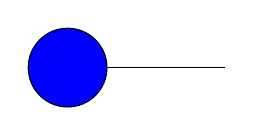
\begin{tikzpicture}
  \draw (0,0) -- (2,0); % Draw a line from (0,0) to (2,0)
  \draw[fill=blue] (0,0) circle (0.5); % Blue filled circle at (0,0)
\end{tikzpicture}
\end{verbatim}

\begin{center}
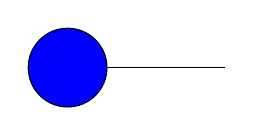
\begin{tikzpicture}
  \draw (0,0) -- (2,0);
  \draw[fill=blue] (0,0) circle (0.5);
\end{tikzpicture}
\end{center}


\subsubsection{Creating a Flowchart}

Example of a simple flowchart:
\begin{verbatim}
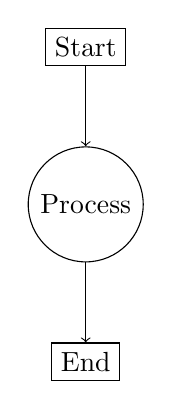
\begin{tikzpicture}[node distance=2cm]
  \node (start) [rectangle, draw] {Start};
  \node (process) [circle, draw, below of=start] {Process};
  \node (end) [rectangle, draw, below of=process] {End};

  \draw[->] (start) -- (process);
  \draw[->] (process) -- (end);
\end{tikzpicture}
\end{verbatim}






\subsubsection{Creating Code Listings with the \texttt{listings} Package}

The `listings' package allows you to display code snippets with syntax highlighting.

Include the package in your preamble:
\begin{verbatim}
\usepackage{listings}
\end{verbatim}

Example of a code listing:
\begin{verbatim}
\begin{lstlisting}[language=Python, caption=Python Example]
def add(a, b):
    return a + b

print(add(2, 3))
\end{lstlisting}
\end{verbatim}

\begin{lstlisting}[language=Python, caption=Python Example]
def add(a, b):
    return a + b

print(add(2, 3))
\end{lstlisting}



\subsection*{Conclusion}

The  `TikZ' and `listings' packages provide powerful tools for academic writing. Whether you need to format units, create complex diagrams, or display code snippets, \LaTeX{} offers a wide range of solutions to meet your needs. With these advanced packages, you can produce polished, professional documents with ease.

\part{Polishing and Publishing}

\section{Customizing \LaTeX{} Output}

Customizing \LaTeX{} output allows you to tailor your document to specific requirements, such as creating shortcuts through custom commands, defining reusable environments, and styling your document for journal submissions. This section covers how to create custom commands and environments, and how to format your document according to journal guidelines.


\subsection{Creating Custom Commands and Environments}

\LaTeX{} allows users to define their own commands and environments, making the writing process more efficient and ensuring consistency across the document.

\subsubsection{Creating Custom Commands}

You can create reusable commands using the `\textbackslash newcommand' syntax. This is useful for repetitive text, symbols, or phrases.

\begin{verbatim}
\newcommand{\R}{\mathbb{R}} % Shortcut for the real numbers symbol
\newcommand{\highlight}[1]{\textbf{#1}} % Bold text shortcut
\end{verbatim}

Usage in the document:
\begin{verbatim}
The set of real numbers is denoted by $\R$. 
This is \highlight{important}.
\end{verbatim}

Output:  
The set of real numbers is denoted by \( \mathbb{R} \).  
This is \textbf{important}.

You can also define commands with optional parameters:
\begin{verbatim}
\newcommand{\unit}[2][m]{#2~\si{#1}}
\end{verbatim}

Usage:  
\begin{verbatim}
\unit[kg]{5} % Output: 5 kg
\end{verbatim}


\subsubsection{Creating Custom Environments}

You can define your own environments using the `\textbackslash newenvironment' command. Custom environments are useful for creating reusable blocks such as definitions or theorems.

Example of a custom environment:
\begin{verbatim}
\newenvironment{definition}[1][Definition]
  {\par\noindent\textbf{#1:} \itshape}
  {\par}
\end{verbatim}

Usage in the document:
\begin{verbatim}
\begin{definition}
A prime number is a natural number greater than 1 that has no positive
divisors other than 1 and itself.
\end{definition}
\end{verbatim}

Output:  
\textbf{Definition:} \textit{A prime number is a natural number greater than 1 that has no positive divisors other than 1 and itself.}


\subsection{Styling for Journal Submissions}

Many academic journals have strict formatting guidelines. \LaTeX{} allows you to style your document according to these requirements by loading specific document classes or defining styles manually.



\subsubsection{Using Journal Templates and Document Classes}

Many journals provide \LaTeX{} templates or document classes. These templates often come with pre-defined formatting for margins, fonts, and citations.

Example of using a journal-specific class:
\begin{verbatim}
\documentclass[12pt,twocolumn]{elsarticle} % Elsevier journal template
\usepackage{hyperref}
\begin{document}
\title{A Study on \LaTeX{} Customization}
\author{John Doe}
\maketitle
\end{document}
\end{verbatim}

In this example, the `elsarticle' class formats the document according to Elsevier’s journal guidelines.



\subsubsection{Customizing Headers, Footers, and Page Layouts}

If your target journal does not provide a specific template, you can use the `geometry' and `fancyhdr' packages to configure your layout.

Example:
\begin{verbatim}
\usepackage[margin=1in]{geometry}
\usepackage{fancyhdr}
\pagestyle{fancy}
\fancyhead[L]{Journal of Examples}
\fancyhead[R]{\thepage}
\fancyfoot[C]{Confidential Submission}
\end{verbatim}

This setup customizes the header to include the journal’s name on the left and the page number on the right, with a footer that displays "Confidential Submission."


\subsubsection{Setting Line Spacing and Font Size}

Use the `setspace' package to adjust line spacing, as required by many journals:
\begin{verbatim}
\usepackage{setspace}
\doublespacing % Set double spacing
\end{verbatim}

You can also use font packages to change the document font if the journal has specific requirements:
\begin{verbatim}
\usepackage{times} % Use Times New Roman
\end{verbatim}


\subsubsection{Adding a Title Page and Abstract}

Most journal submissions require a title page and an abstract. You can create a title page using the following commands:
\begin{verbatim}
\title{A Study on Custom \LaTeX{} Output}
\author{John Doe \\ Department of Mathematics, University of Examples}
\date{\today}
\maketitle
\begin{abstract}
This study explores methods for customizing \LaTeX{} output,
including creating custom commands and environments.
\end{abstract}
\end{verbatim}

This will generate a title page followed by an abstract, formatted according to typical journal submission standards.



\subsubsection{Including a Bibliography with BibLaTeX}

Many journals require specific citation styles. Use the `biblatex' package to manage your references:
\begin{verbatim}
\usepackage[backend=biber,style=apa]{biblatex}
\addbibresource{references.bib}
\end{verbatim}

This example applies the APA citation style. You can change the style to meet journal requirements, such as IEEE or Chicago.



\subsection*{Conclusion}

Customizing \LaTeX{} output is essential for meeting the requirements of academic journals and ensuring consistency in your document. Creating custom commands and environments streamlines your workflow, while \LaTeX’s flexibility allows you to style your document for specific journal submissions. With these tools, you can produce high-quality documents tailored to any publication’s standards.

\section{Exporting and Publishing}

Once your \LaTeX{} document is complete, you’ll need to export it to a distributable format, often as a PDF, and prepare it for submission or collaboration. This section covers the process of exporting PDFs, preparing your document for journal or conference submissions, and using Overleaf for collaborative writing.


\subsection{Exporting PDFs and Sharing Documents}

PDF is the most common output format for \LaTeX{} documents, especially for academic and professional publishing. Exporting to PDF ensures that your document looks the same on any device and platform.

\subsubsection{Exporting to PDF Using Your Editor}

Most \LaTeX{} editors provide a simple way to compile and export your document to PDF:
\begin{itemize}

\item \textbf{Overleaf:} Click the \textbf{Recompile} button to generate a PDF.
\item \textbf{TeXstudio:} Use the shortcut `F5' or click \textbf{Build \& View}.
\item \textbf{VSCode:} Use the `Ctrl + Alt + B' (or `Cmd + Alt + B' on macOS) shortcut to compile with the \LaTeX{} Workshop extension.
\end{itemize}

\subsubsection{Exporting from the Command Line}

You can also compile your \LaTeX{} file from the command line:

\begin{verbatim}
pdflatex mydocument.tex
\end{verbatim}

If you are using `biblatex' with `biber', follow this sequence:

\begin{verbatim}
pdflatex mydocument.tex
biber mydocument
pdflatex mydocument.tex
pdflatex mydocument.tex
\end{verbatim}

This ensures that all citations and cross-references are processed correctly.

\subsubsection{Sharing Your PDF Document}

Once your PDF is ready, you can share it via:

\begin{itemize}


\item \textbf{Email}: Attach the PDF to an email.
\item \textbf{Cloud Storage}: Upload to Google Drive, Dropbox, or OneDrive.
\item \textbf{GitHub or GitLab}: Share it through a version control platform if you are working on a collaborative project.

\end{itemize}

\subsection{Preparing for Journal or Conference Submissions}

When submitting to a journal or conference, it’s important to follow the formatting guidelines provided by the publisher or organizer. Here are some key steps to ensure your document meets submission requirements.

\subsubsection{Using Journal or Conference Templates}

Many journals and conferences provide \LaTeX{} templates to ensure uniform formatting. Search the journal’s website or conference portal for the appropriate template. Some examples include:

\begin{itemize}


\item \textbf{Elsevier Journals}: Use the `elsarticle' template.
\item \textbf{IEEE Conferences}: Use the `ieeeconf' template.
\item \textbf{ACM Journals}: Use the `acmart' template.
\end{itemize}

Example using the IEEE template:
\begin{verbatim}
\documentclass[conference]{IEEEtran}
\title{A Study on Exporting and Publishing}
\author{John Doe}
\date{}

\begin{document}
\maketitle
\begin{abstract}
This paper discusses exporting \LaTeX{} documents and preparing them for publication.
\end{abstract}
\end{document}
\end{verbatim}

\subsubsection{Reviewing Guidelines}

Ensure that your document follows the submission guidelines, including:

\begin{itemize}


\item \textbf{Margins and Spacing}: Use the appropriate layout settings.
\item \textbf{File Format}: Submit in PDF unless otherwise specified.
\item \textbf{Bibliography Style}: Use the correct citation style (e.g., APA, IEEE).
\item \textbf{Plagiarism Check}: Some journals require plagiarism screening before submission.
\end{itemize}

\subsubsection{Handling Revisions and Resubmissions}

If your submission requires revisions, make the necessary changes in \LaTeX{} and regenerate the PDF. Use version control (e.g., Git) to track changes and resubmit your updated document.



\subsection{Using Overleaf for Collaborative Writing}

Overleaf is a cloud-based \LaTeX{} editor that makes it easy to collaborate on \LaTeX{} projects in real-time. It provides an intuitive interface and supports seamless sharing with co-authors.

\subsubsection{Creating a Project on Overleaf}

\begin{enumerate}



\item  Go to \url{https://overleaf.com} and create an account.
\item Click \textbf{New Project} and choose:
 \begin{itemize}


   \item \textbf{Blank Project}: Start from scratch.
   \item \textbf{Upload Project}: Upload existing \LaTeX{} files.
   \item \textbf{From a Template}: Use a journal or conference template.
\end{itemize}
\end{enumerate}
\subsubsection{Sharing Your Project with Co-Authors}

To collaborate with others:

\begin{enumerate}


\item Open your project.
\item Click \textbf{Share} at the top right.
\item Enter the email addresses of your collaborators and set permissions (e.g., read-only or edit access).
\end{enumerate}
Your collaborators will receive an email invitation to join the project.

\subsubsection{Real-Time Collaboration}

Overleaf supports real-time editing, meaning multiple authors can work on the same document simultaneously. Changes are reflected immediately, and Overleaf tracks the version history of the project.

\subsubsection{Compiling and Exporting in Overleaf}

Overleaf automatically compiles your document when changes are made. You can download the final PDF by clicking \textbf{Download PDF}.

\subsubsection{Integrating Overleaf with GitHub}

Overleaf can sync with GitHub for version control:

\begin{enumerate}
    \item In Overleaf, go to \textbf{Menu $>$ GitHub}.
    \item Connect your GitHub account and select a repository.
    \item Push or pull changes between Overleaf and GitHub.
\end{enumerate}


\subsection*{Conclusion}

Exporting and publishing \LaTeX{} documents is an essential part of academic writing. Whether you are submitting to a journal or collaborating with co-authors, \LaTeX{} offers robust tools to ensure your document is polished and ready for distribution. Using Overleaf simplifies collaboration, while following journal guidelines ensures that your work meets submission requirements. With the right tools and workflows, you can efficiently manage the publishing process from start to finish.



\section{Templates for Common Academic Documents}

Using templates simplifies the process of formatting academic documents, ensuring they meet institutional or journal requirements. This section covers templates for research papers, theses/dissertations, and presentations with Beamer. Each template provides a starting point with appropriate formatting, layout, and structure.


\subsection{Research Paper Template}

A research paper template follows common formatting requirements such as title pages, abstract, sections, citations, and references. The following template demonstrates the typical structure for an article.

\subsubsection{Basic Research Paper Template}

\begin{verbatim}
\documentclass[12pt]{article}
\usepackage{amsmath, graphicx, hyperref, natbib}

\title{A Comprehensive Study on \LaTeX{} Templates}
\author{John Doe \\ Department of Computer Science, Example University}
\date{\today}

\begin{document}
\maketitle

\begin{abstract}
This paper discusses the use of \LaTeX{} templates for academic writing,
including research papers, theses, and presentations.
\end{abstract}

\section{Introduction}
\LaTeX{} offers various templates for academic writing to streamline the
formatting process. This paper demonstrates the structure of a typical
research paper.

\section{Methodology}
The methodology section describes the research approach.

\section{Results}
The results section presents the findings.

\section{Conclusion}
This paper highlights the benefits of using \LaTeX{} templates.

\bibliographystyle{plain}
\bibliography{references}
\end{document}
\end{verbatim}

\subsubsection{Explanation}
\begin{itemize}


\item \textbf{Title and Author Information}: `\textbackslash title', `\textbackslash author', and `\textbackslash date' define the title page.
\item \textbf{Abstract}: The `abstract' environment provides a summary of the paper.
\item \textbf{Sections}: `\textbackslash section' commands divide the paper into logical sections.
\item \textbf{References}: Use the `natbib' package to manage citations, and include a '.bib' file for the bibliography.

\end{itemize}
\subsection{Thesis/Dissertation Template}

Theses and dissertations typically require a more complex structure, including a title page, abstract, acknowledgments, table of contents, and chapters.

\subsubsection{Basic Thesis/Dissertation Template}

\begin{verbatim}
\documentclass[12pt]{report}
\usepackage{graphicx, hyperref, setspace}

\title{A Sample Thesis Template}
\author{John Doe}
\date{\today}

\begin{document}
\maketitle

\begin{abstract}
This thesis demonstrates how to use \LaTeX{} templates for dissertations.
\end{abstract}

\chapter*{Acknowledgments}
I would like to thank everyone who supported me during my research.

\tableofcontents

\chapter{Introduction}
This chapter introduces the thesis and its objectives.

\chapter{Literature Review}
This chapter discusses previous work in the field.

\chapter{Methodology}
Details about the research methodology used in the thesis.

\chapter{Results}
Presentation of results obtained from the research.

\chapter{Conclusion}
Summary of findings and suggestions for future work.

\bibliographystyle{plain}
\bibliography{references}

\appendix
\chapter{Appendix}
This appendix contains supplementary material.
\end{document}
\end{verbatim}

\subsubsection{Explanation}

\begin{itemize}


\item \textbf{Chapters}: Use `\textbackslash chapter' to organize the content into logical sections.
\item \textbf{Table of Contents}: Automatically generated with `\textbackslash tableofcontents'.
\item \textbf{Appendix}: Use `\textbackslash appendix' to add supplementary materials.
\item \textbf{Line Spacing}: Add `\textbackslash doublespacing' from the `setspace' package if required.

\end{itemize}

\subsection{Presentation with Beamer}

The Beamer class is used to create high-quality presentations directly in \LaTeX{}. It provides tools to format slides, include figures, and animate content.

\subsubsection{Basic Beamer Presentation Template}

\begin{verbatim}
\documentclass{beamer}
\usepackage{graphicx}

\title{A \LaTeX{} Presentation on Templates}
\author{John Doe}
\date{\today}

\begin{document}

\frame{\titlepage}

\begin{frame}{Outline}
\tableofcontents
\end{frame}

\section{Introduction}
\begin{frame}{Introduction}
This presentation discusses how to use templates in \LaTeX{}.
\end{frame}

\section{Research Paper Template}
\begin{frame}{Research Paper Template}
A structured template simplifies the writing process.
\end{frame}

\section{Thesis/Dissertation Template}
\begin{frame}{Thesis/Dissertation Template}
Thesis templates include chapters, abstract, and acknowledgments.
\end{frame}

\section{Conclusion}
\begin{frame}{Conclusion}
Using \LaTeX{} templates ensures consistency and professionalism.
\end{frame}

\end{document}
\end{verbatim}

\subsubsection{Explanation}

\begin{itemize}


\item \textbf{Title Page}: Automatically generated using `\textbackslash titlepage'.
\item \textbf{Table of Contents}: The `\textbackslash tableofcontents' command creates an outline slide.
\item \textbf{Sections and Frames}: Use `\textbackslash section' and `\textbackslash frame' for slide content.

\end{itemize}

\subsection*{Conclusion}

Templates simplify the creation of academic documents by ensuring consistent formatting and structure. Whether you are working on a research paper, thesis, or presentation, \LaTeX{} provides a range of templates to meet your needs. These templates ensure that your work meets academic standards while reducing the time spent on formatting.



\part{Using VSCode, Github, and Zotero with \LaTeX}


\section{Setting Up VSCode to Use with \LaTeX{}}

Visual Studio Code (VSCode) is a powerful, free code editor that can be used for \LaTeX{} with the help of extensions. This is the \LaTeX{} editor that I use to prepare all of my documents. Below are step-by-step instructions to set up VSCode for \LaTeX{} development.

\subsection{Step 1: Install VSCode}
If you don’t already have VSCode installed, download it from the official website:  
\url{https://code.visualstudio.com/}  
Follow the installation instructions for your operating system (Windows, macOS, or Linux).

\subsection{Step 2: Install a LaTeX Distribution}
Ensure you have a \LaTeX{} distribution installed. Choose one based on your platform:  
\begin{itemize}
    \item \textbf{TeX Live}: Suitable for Linux and cross-platform users  
          \url{https://www.tug.org/texlive/}
    \item \textbf{MiKTeX}: Recommended for Windows users  
          \url{https://miktex.org/}
    \item \textbf{MacTeX}: Best for macOS users  
          \url{https://tug.org/mactex/}
\end{itemize}

\subsection{Step 3: Installing Perl on Windows}

Some features of \LaTeX{} distributions, such as \textbf{TeX Live}, rely on Perl scripts for important tasks, including package management and updates. If you are using \TeX{} Live on Windows and working with VSCode, you may encounter errors indicating that Perl is missing. Follow the steps below to install Perl and ensure your \LaTeX{} setup works smoothly.

\subsubsection*{Check if Perl is Installed}

To see if Perl is already installed on your system:
\begin{enumerate}
    \item Open the \texttt{Command Prompt} by typing \texttt{cmd} in the search bar.
    \item Type the following command:
\end{enumerate}

\begin{verbatim}
perl --version
\end{verbatim}

If Perl is installed, this command will display the version number. If it is not installed, you will need to download and install it.

\subsubsection*{Install Perl on Windows}

\begin{itemize}
    \item Visit the official Strawberry Perl website:  
    \url{https://strawberryperl.com/}
    \item Download the latest version of Strawberry Perl, which provides a complete Perl environment for Windows.
    \item Run the installer and follow the on-screen instructions.
    \item Ensure that the option to \textbf{add Perl to the PATH environment variable} is checked during installation.
\end{itemize}

\subsubsection*{Verify the Installation}

After installation, verify that Perl is correctly set up:
\begin{enumerate}
    \item Open the \texttt{Command Prompt} again.
    \item Run the following command:
\end{enumerate}

\begin{verbatim}
perl --version
\end{verbatim}

If the installation was successful, you should see the version number of Perl displayed.

\subsubsection*{Ensure VSCode Can Use Perl}

VSCode relies on your system’s PATH variable to find installed tools. If Perl was added to the PATH during installation, VSCode should now be able to access it. Restart both VSCode and your computer to ensure the changes take effect.

\subsection*{Troubleshooting Tips}

\begin{itemize}
    \item If you still encounter issues, make sure Perl is correctly listed in the PATH. You can verify this by running the following command in the Command Prompt:
\end{itemize}

\begin{verbatim}
echo %PATH%
\end{verbatim}

\begin{itemize}
    \item If Perl is not listed, add it manually to the PATH via:
          \texttt{Control Panel} $\rightarrow$ \texttt{System} $\rightarrow$ \texttt{Advanced System Settings} $\rightarrow$ \texttt{Environment Variables}.
\end{itemize}





\subsection{Step 4: Install the \LaTeX{} Workshop Extension}
The \textbf{\LaTeX{} Workshop} extension provides all the necessary tools to write, compile, and preview \LaTeX{} documents in VSCode.
\begin{enumerate}
    \item Open VSCode.
    \item Click on the \textbf{Extensions} icon on the left sidebar (or press \texttt{Ctrl+Shift+X}).
    \item Search for \textbf{\LaTeX{} Workshop} and click \textbf{Install}.
\end{enumerate}

\subsection{Step 5: Configure the \LaTeX{} Workshop Extension}
The \LaTeX{} Workshop extension provides many features, including PDF preview, syntax highlighting, and automatic compilation. You may need to adjust some settings to ensure smooth operation.

\begin{enumerate}
    \item Open the Command Palette (\texttt{Ctrl+Shift+P} or \texttt{Cmd+Shift+P} on macOS).
    \item Search for \texttt{Preferences: Open Settings (JSON)}.
    \item Add the following configuration to your \texttt{settings.json} file to customize the build process:
\end{enumerate}

\begin{verbatim}
"latex-workshop.latex.tools": [
    {
        "name": "pdflatex",
        "command": "pdflatex",
        "args": [
            "-synctex=1",
            "-interaction=nonstopmode",
            "-file-line-error",
            "%DOC%"
        ]
    }
],
"latex-workshop.latex.recipes": [
    {
        "name": "pdflatex",
        "tools": ["pdflatex"]
    }
]
\end{verbatim}

This configuration ensures that VSCode uses \texttt{pdflatex} to compile your documents with error reporting and SyncTeX enabled for PDF synchronization. Alternatively you can see and copy my \texttt{settings.json} code in my GitHub Repository: \url{https://github.com/derronborders/adultlearninglatex.git}

\subsection{Step 6: Verify the Setup with a Sample Document}
To test your setup:
\begin{enumerate}
    \item Create a new file in VSCode and save it as \texttt{hello\_world.tex}.
    \item Type the following \LaTeX{} code:
\end{enumerate}

\begin{verbatim}
\documentclass{article}
\begin{document}
Hello, world!
\end{document}
\end{verbatim}

\begin{enumerate}
    \item Press \texttt{Ctrl+Alt+B} (or \texttt{Cmd+Alt+B} on macOS) to build the document.
    \item The PDF output should appear in the preview pane.
\end{enumerate}

\subsection{Step 7: Troubleshooting Common Issues}
\begin{itemize}
    \item If VSCode cannot find the \texttt{pdflatex} command, ensure that the \LaTeX{} distribution is installed correctly and that the path to its binaries is included in your system's \texttt{PATH} variable.
    \item If the PDF preview does not appear, try restarting VSCode and ensure that the \texttt{latex-workshop.latex.recipes} configuration is correct.
\end{itemize}

\subsection{Other Useful Extensions}

There are other useful \LaTeX{} extensions that one can use in VSCode. Another one that I use is \texttt{LTeX+ - LanguageTool grammar/spell checking}, which is useful for catching basic spelling and grammar errors. 


\section{Using VSCode with GitHub for \LaTeX{} Projects}

In this section, I will guide you through the process of integrating VSCode with GitHub to back up and collaborate on your \LaTeX{} projects. GitHub provides a version control system that ensures your work is safely stored and allows you to work with others efficiently.

\subsection{Step 1: Install Git}

First, make sure you have \textbf{Git} installed, as it is required to use GitHub. 
\begin{enumerate}
    \item Download Git from the official website:  
    \url{https://git-scm.com/}
    \item Run the installer and select the default options.
    \item Verify the installation by opening the \texttt{Command Prompt} or \texttt{Terminal} and typing:
\end{enumerate}

\begin{verbatim}
git --version
\end{verbatim}

If Git is installed correctly, this command will display the version number.

\subsection{Step 2: Set Up a GitHub Account}

\begin{itemize}
    \item Go to \url{https://github.com/} and sign up for a free GitHub account if you don’t have one.
    \item Once signed in, click on \textbf{Repositories} $\rightarrow$ \textbf{New} to create a new repository.
    \item Give the repository a name (e.g., \texttt{MyLaTeXProject}) and select the option \textbf{Initialize this repository with a README}.
\end{itemize}

\subsection{Step 3: Install the GitHub Extension for VSCode}

\begin{enumerate}
    \item Open VSCode.
    \item Click on the \textbf{Extensions} icon (or press \texttt{Ctrl+Shift+X}).
    \item Search for \textbf{GitHub Repositories} and install it.
\end{enumerate}

\subsection{Step 4: Configure Git in VSCode}

\begin{enumerate}
    \item Open the \texttt{Command Palette} in VSCode (\texttt{Ctrl+Shift+P} or \texttt{Cmd+Shift+P} on macOS).
    \item Type \texttt{Git: Clone} and press \texttt{Enter}.
    \item Paste the URL of your GitHub repository (e.g., \texttt{https://github.com/username/MyLaTeXProject.git}).
    \item Choose a local folder where the repository will be cloned.
\end{enumerate}

\subsection{Step 5: Initialize a Git Repository for Your Project}

If your project is not yet connected to Git:
\begin{enumerate}
    \item Open your \LaTeX{} project folder in VSCode.
    \item Open the \texttt{Terminal} within VSCode (\texttt{Ctrl+`}) and type:
\end{enumerate}

\begin{verbatim}
git init
git add .
git commit -m "Initial commit"
\end{verbatim}

This initializes the Git repository and commits all current files.

\subsection{Step 6: Push Your Project to GitHub}

\begin{enumerate}
    \item Add your GitHub repository as a remote by typing:
\end{enumerate}

\begin{verbatim}
git remote add origin https://github.com/username/MyLaTeXProject.git
git branch -M main
git push -u origin main
\end{verbatim}

This command uploads your project to GitHub.

\subsection{Step 7: Back Up Your Work with Regular Commits}

As you make changes to your \LaTeX{} project:
\begin{enumerate}
    \item Use the following commands to save your changes:
\end{enumerate}

\begin{verbatim}
git add .
git commit -m "Describe your changes"
git push
\end{verbatim}

These commands stage, commit, and push your changes to GitHub.

\subsection{Step 8: Collaborate with Others}

Collaborating on a project is simple with GitHub:
\begin{itemize}
    \item Share your repository’s URL with collaborators.
    \item They can clone the repository using the \texttt{Git: Clone} command in VSCode.
    \item Collaborators can create their own branches using:
    \begin{verbatim}
    git checkout -b new-branch-name
    \end{verbatim}
    \item Changes can be merged into the main branch through \textbf{pull requests} on GitHub.
\end{itemize}

\subsection{Step 9: Handle Merge Conflicts}

Merge conflicts can occur when multiple people edit the same part of a document. Use these steps to resolve conflicts:
\begin{enumerate}
    \item Pull the latest changes from GitHub:
    \begin{verbatim}
    git pull
    \end{verbatim}
    \item If a conflict occurs, VSCode will highlight the conflicting sections.
    \item Choose the correct version or manually merge the changes.
    \item After resolving the conflict, commit the changes:
    \begin{verbatim}
    git add .
    git commit -m "Resolved merge conflict"
    git push
    \end{verbatim}
\end{enumerate}

\section{Utilizing Zotero to Manage References and Integrate with LaTeX}

Zotero is a powerful reference management tool that helps organize research materials, generate citations, and create bibliographies. It integrates seamlessly with \LaTeX{} through the Better BibTeX extension, allowing users to export `.bib' files of their libraries for use in \LaTeX{} documents. This section provides a step-by-step guide to managing references with Zotero and using Better BibTeX to generate `.bib' files.


\subsection{Setting Up Zotero for Reference Management}

Zotero simplifies reference management by allowing users to store and organize citations, PDFs, and notes in one place.

\subsubsection{Installing Zotero}

\begin{enumerate}


\item Go to \url{https://www.zotero.org/} and download Zotero.
\item Install the application following the on-screen instructions.
\item  Create an account to enable syncing and cloud backups.
\end{enumerate}
\subsubsection{Adding References to Zotero}

There are several ways to add references to your Zotero library:
\begin{enumerate}
    \item \textbf{Manually}: Click the green \textbf{+} icon and select \textbf{Book, Article, or Other Item} to add details manually.
    \item \textbf{Web Browser Plugin}: Install the Zotero Connector plugin for your browser to quickly add items from websites, databases, and journals.
    \item \textbf{Import Files}: Drag and drop PDFs or other documents into the Zotero interface. Zotero can extract metadata to create a reference entry.
\end{enumerate}


Organize references into \textbf{collections} or \textbf{tags} to manage them effectively.


\subsection{Integrating Zotero with Better BibTeX for \LaTeX{}}

Better BibTeX (BBT) is a Zotero plugin that enhances the export of `.bib' files and ensures compatibility with \LaTeX.

\subsubsection{Installing Better BibTeX}

\begin{enumerate}
    \item Open Zotero and go to \textbf{Tools $>$ Add-ons}.
    \item In the Add-ons Manager, click \textbf{Get Add-ons} and search for \textbf{Better BibTeX} (or download it from \url{https://retorque.re/zotero-better-bibtex/}).
    \item Restart Zotero to enable Better BibTeX.
\end{enumerate}


\subsubsection{Creating a .bib File of Your Zotero Library}

Once Better BibTeX is installed, follow these steps to export your Zotero references as a `.bib' file:

\begin{enumerate}
    \item Right-click a \textbf{collection} or \textbf{individual reference} in Zotero.
    \item Select \textbf{Export Library} or \textbf{Export Item}.
    \item Choose \textbf{Better BibTeX} from the export format options.
    \item Save the `.bib' file in the same directory as your \LaTeX{} project.
\end{enumerate}




\subsubsection{Generating a Dynamic .bib File with Auto-Export}

Better BibTeX also supports \textbf{automatic exports} to keep your `.bib' file synchronized with Zotero. This is useful when you are actively adding references to your library during a project.

\begin{enumerate}
    \item In Zotero, go to \textbf{Tools $>$ Preferences $>$ Better BibTeX}.
    \item Under the \textbf{Automatic Export} tab, click \textbf{New Auto-export}.
    \item Choose a \textbf{collection} and set the export format to \textbf{Better BibTeX}.
    \item Select a destination for the `.bib' file. Ensure that it matches the directory of your \LaTeX{} project.
    \item  Enable \textbf{Auto-Export on Change} to keep the `.bib' file updated automatically.
\end{enumerate}


\subsection{Using Zotero-Generated .bib Files in \LaTeX}

After creating the `.bib' file, follow these steps to use it in your \LaTeX{} document:

\subsubsection{Adding the .bib File to Your Project}

\begin{enumerate}
    \item Place the `.bib' file in the same directory as your \LaTeX{} source file.
    \item In your \LaTeX{} document preamble, add:\\
    \begin{verbatim}
        \usepackage[backend=biber,style=apa]{biblatex}
        \addbibresource{references.bib}
        \end{verbatim}
        
\end{enumerate}



\subsubsection{Citing References in \LaTeX{}}

Use the `\textbackslash cite' or `\textbackslash textcite' commands to cite references:
\begin{verbatim}
\cite{lamport1994} % Inline citation
\textcite{knuth1986} % In-text citation with author name
\end{verbatim}


\subsubsection{Compiling Your Document with Biber}

If you are using `biblatex' with Better BibTeX, follow this compilation sequence:

\begin{verbatim}
pdflatex mydocument.tex
biber mydocument
pdflatex mydocument.tex
pdflatex mydocument.tex
\end{verbatim}

This ensures that citations and bibliographies are correctly processed.


\subsection{Troubleshooting Zotero-LaTeX Integration}

Here are some common issues and solutions:

\begin{itemize}
    \item \textbf{Missing Bibliography Entries}: Ensure that the `.bib' file is correctly linked in the \LaTeX{} document using `\textbackslash addbibresource'.
    \item \textbf{Biber Errors}: Verify that the compilation sequence includes `biber' if you are using `biblatex'.
    \item \textbf{Duplicate Entries}: Use the Zotero \textbf{Duplicate Items} feature to merge duplicate references before exporting the `.bib' file.
\end{itemize}

\subsection*{Conclusion}

Using Zotero with Better BibTeX simplifies reference management and ensures smooth integration with \LaTeX{}. By exporting `.bib' files from Zotero, you can maintain an organized bibliography and efficiently cite sources in your \LaTeX{} projects. Auto-export features in Better BibTeX further streamline the process, keeping your bibliography up-to-date with minimal effort.

\newpage

\begin{appendices}
    \section{Additional Resources}

    There are so many resources out there to help you on your journey of mastering \LaTeX. Whenever you run into an issue, it is very likely you are not the first one to have this issue. The first thing I do is run to Google and ask my question.

    Below are some additional resources that you can turn to when you are looking to typset something in a certain way and do not know.

    \begin{itemize}
        \item \url{www.ctan.org} - Most of the packages that are created for \LaTeX{} are archived on this website. If you are having trouble with a certain package, going to that package's documentation is a good start.
        \item \url{www.overleaf.com} - Overleaf has a lot of tutorials on how to do things with a lot of examples. You can also find a ton of templates on there as well.
        \item \url{tex.stackexchange.com} - This website is invaluable and without it I would not have been able to finish my thesis in \LaTeX{}. There are a lot of knowledgeable people on here and if you put the effort into asking your questions, they will put the effort into helping you. Most times, someone has already asked the question I'm looking for, so make sure it is in your bookmarks!
        \item \url{www.reddit.com/r/latex} - R/Latex is a good place to ask questions or search for solutions for to just discuss \LaTeX{} in general.
        \item \url{https://github.com/derronborders/adultlearninglatex.git} - I created this GitHub repository to provide templates and other additional resources for using \LaTeX{} including the files for creating this manual.
    \end{itemize}

\end{appendices}

\end{document}